\documentclass[11pt,a4paper]{article}

\usepackage[spanish,es-nodecimaldot]{babel}
\usepackage[T1]{fontenc}
\usepackage[utf8]{inputenc}
\usepackage{lmodern}
\usepackage{geometry}
\usepackage{graphicx}
\usepackage{float}
\usepackage{hyperref}
\usepackage{enumitem}

\geometry{margin=2.5cm}
\hypersetup{colorlinks=true,linkcolor=black,urlcolor=blue}
\graphicspath{{img/}}

\title{Captura de paquetes con tcpdump y Wireshark}
\author{Javier Siñuka}
\date{20 de septiembre de 2026}

\begin{document}
\maketitle

\section{Objetivo}

Capturar paquetes en la PC y mostrarlos en Wireshark. Para ello se utilizó
\texttt{tcpdump} para guardar tráfico real en un archivo \texttt{.pcap} y luego
se abrió ese mismo archivo en Wireshark para observar los protocolos y el
contenido de una comunicación de prueba.

\section{Entorno utilizado}

La captura se realizó el 20 de septiembre de 2026 en un contenedor temporal
Ubuntu 24.04 dentro de la PC.
Se inició un servidor HTTP en \texttt{127.0.0.1:8080} y se realizó una petición
con \texttt{curl}. Se capturó la interfaz de retorno local \texttt{lo} del
contenedor: por lo tanto, ambos extremos tienen la dirección
\texttt{127.0.0.1}. El tráfico corresponde a una comunicación local real y no
a una conexión externa por Wi-Fi. Las imágenes son capturas de las aplicaciones
ejecutadas en un escritorio virtual del mismo entorno.

\section{Procedimiento realizado}

\subsection{Captura con tcpdump}

Se inició el servidor de prueba y se ejecutó el siguiente comando con permisos
de captura:

\begin{verbatim}
tcpdump -i lo -nn -s 0 -U \
  -w evidencias/captura_http.pcap 'tcp port 8080'
\end{verbatim}

\begin{itemize}[noitemsep]
    \item \texttt{-i lo}: selecciona la interfaz de retorno local.
    \item \texttt{-nn}: evita resolver nombres de equipos y de servicios.
    \item \texttt{-s 0}: permite guardar los paquetes completos.
    \item \texttt{-U}: vuelca cada paquete al archivo a medida que se captura.
    \item \texttt{-w}: indica el archivo de salida.
    \item \texttt{tcp port 8080}: limita la captura al servicio de prueba.
\end{itemize}

Mientras tcpdump estaba activo se generó la comunicación:

\begin{verbatim}
curl --noproxy '*' http://127.0.0.1:8080/
\end{verbatim}

Luego se detuvo la captura con la señal de interrupción, equivalente a
\texttt{Ctrl+C}, y se consultó el archivo mediante
\texttt{tcpdump -nn -r evidencias/captura\_http.pcap}.
La Figura~\ref{fig:tcpdump} muestra la lectura real del archivo y el resumen
del proceso de captura.

\begin{figure}[H]
    \centering
    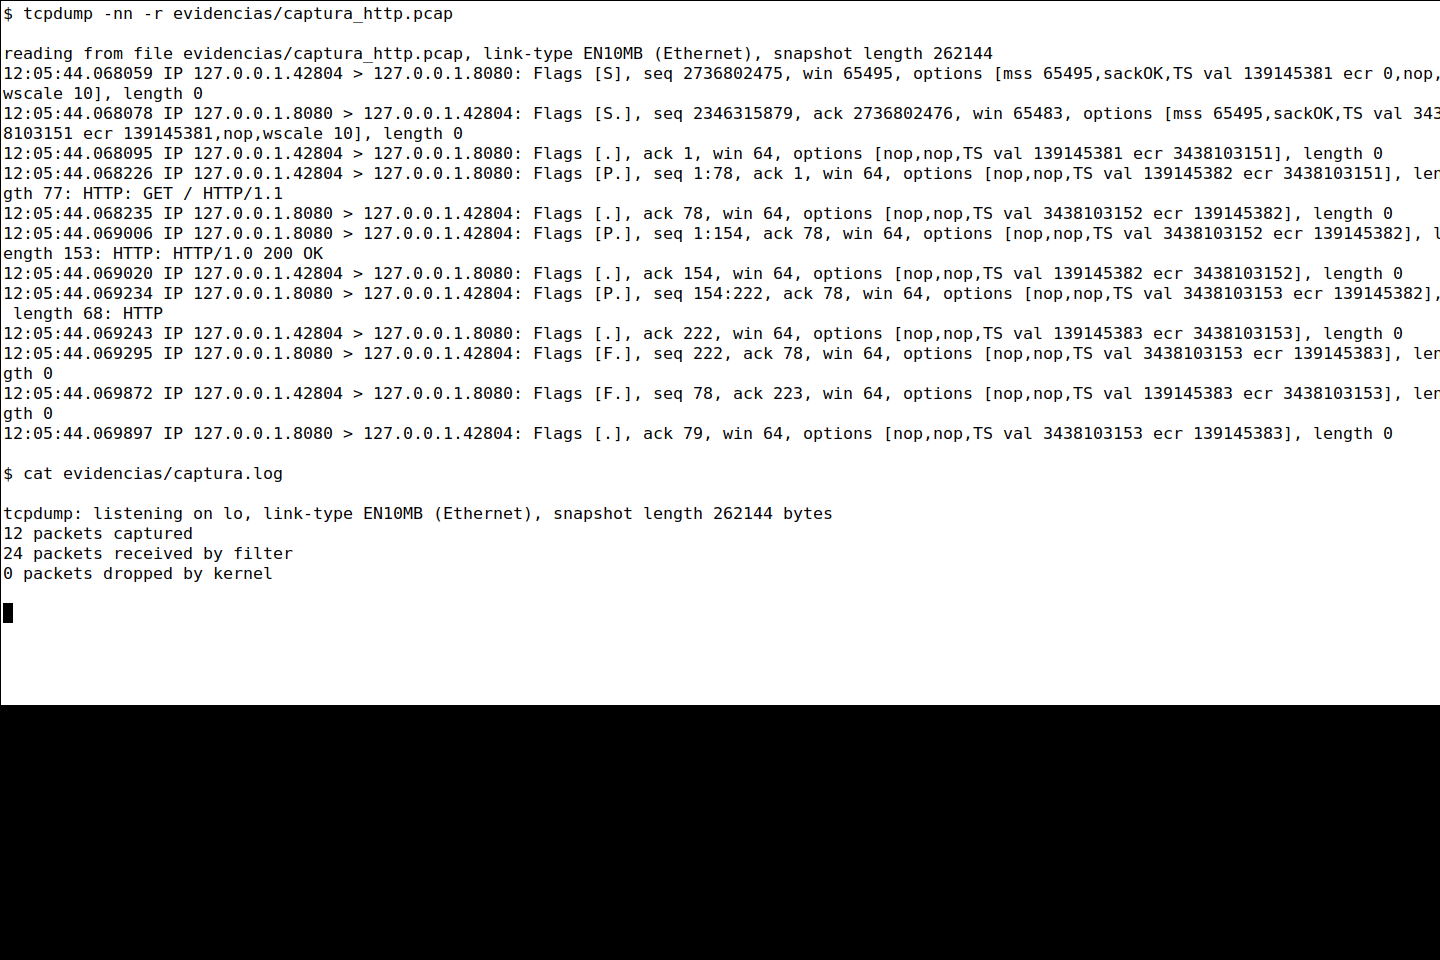
\includegraphics[width=\textwidth,trim=0 258bp 0 0,clip]{tcpdump.png}
    \caption{Terminal con la salida de tcpdump correspondiente al tráfico HTTP
    local capturado y el resumen de captura.}
    \label{fig:tcpdump}
\end{figure}

\subsection{Visualización en Wireshark}

Se abrió \texttt{evidencias/captura\_http.pcap} en Wireshark y se aplicó el
filtro de visualización \texttt{tcp.port == 8080}. Este filtro muestra los
paquetes del puerto utilizado por el servidor. A diferencia del filtro de
captura de tcpdump, actúa sobre los paquetes ya guardados.

En el panel superior se observa la secuencia de paquetes; en el panel inferior izquierdo,
los campos del paquete seleccionado; y a su derecha, los bytes. La
Figura~\ref{fig:wireshark} muestra el mismo intercambio registrado con tcpdump.

\begin{figure}[H]
    \centering
    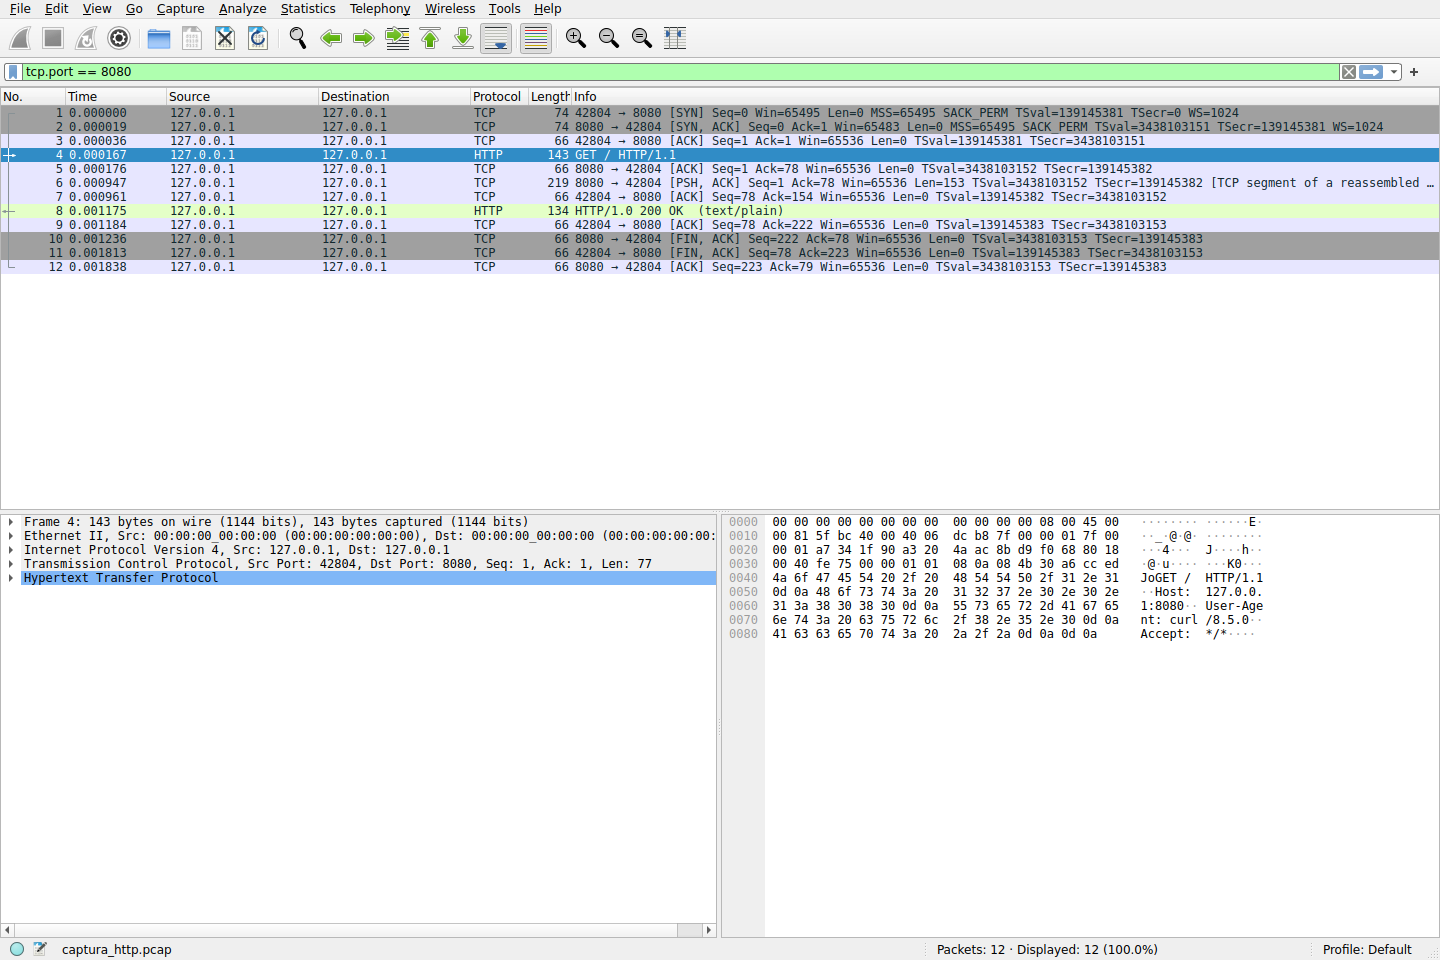
\includegraphics[width=\textwidth]{wireshark.png}
    \caption{Archivo de captura abierto en Wireshark, con el filtro del puerto
    8080 y una petición HTTP seleccionada.}
    \label{fig:wireshark}
\end{figure}

\section{Resultados y conclusión}

Se registraron 12 paquetes y tcpdump informó 0 paquetes descartados por el
núcleo. En la captura se identifica el establecimiento de la conexión TCP mediante
los paquetes \texttt{SYN}, \texttt{SYN, ACK} y \texttt{ACK}. A continuación
aparece la petición \texttt{GET / HTTP/1.1} y la respuesta del servidor
\texttt{HTTP/1.0 200 OK}. Finalmente se observan los paquetes de cierre de la
conexión, con las banderas \texttt{FIN} y \texttt{ACK}.

Como se utilizó HTTP sin TLS, el contenido de la petición y la respuesta se
puede leer en la captura. Esto permite reconocer la diferencia entre capturar
paquetes y proteger su contenido: la captura registra el tráfico, mientras que
el cifrado impediría leer directamente los datos de aplicación sin las claves
correspondientes.

\end{document}
